\section{Hit Rate Is Not a Performance Model}
\label{sec:performance-model}

The replay results naturally use hit rate because they ask which accesses would have been served from resident memory. End-to-end performance, however, depends on the \emph{time} exposed by misses. Two complications prevent miss count from being a sufficient performance model: the runtime's hit counter has non-obvious semantics, and the time cost of a miss changes with I/O concurrency.

\begin{figure}[t]
    \centering
    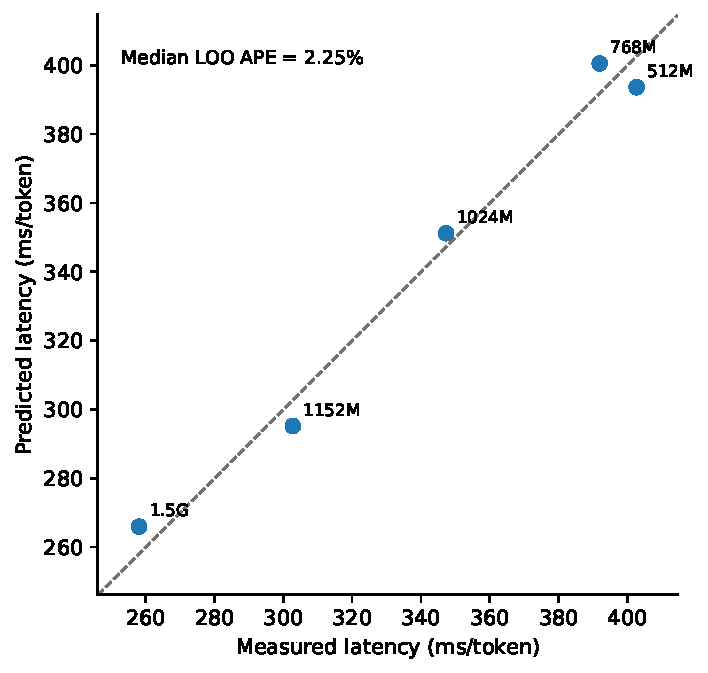
\includegraphics[width=0.72\linewidth]{../experiments/EXP-025-performance-model/figures/performance_model_predicted_vs_measured.pdf}
    \caption{Interpretable prediction of token latency. Measured versus leave-one-configuration-out predicted latency for the five preregistered 30B memory configurations. The dashed diagonal denotes perfect prediction. Median absolute percentage error is 2.25\%, below the preregistered 15\% criterion. The result supports the predictive usefulness of the latency decomposition over the tested configurations, without separately identifying every physical latency component.}
    \label{fig:performance-model}
\end{figure}

\subsection{Runtime hit accounting and expert reuse are different quantities}

In the evaluated expert store, the gate, up, and down nodes request the slices associated with an expert, but misses occur when the first node loads those slices; subsequent nodes re-pin them and hit. EXP-020 and EXP-021 establish this behavior record-for-record. Across the 252 qualified EXP-007 runs, the expert-level gate-slice miss rate is exactly three times the runtime-style miss rate.

Consequently, a runtime hit rate near 90\% does not imply a 90\% expert-level reuse rate. For example, on qualified 30B coding runs the workload-only expert-level hit rates are 70.60\%, 49.75\%, and 41.46\% at 4, 2, and 1.5\,GiB, while the corresponding runtime-style rates are 90.2\%, 83.2\%, and 80.5\%. The distinction is mechanical rather than statistical and is preserved throughout this paper.

This also separates the runtime metrics from the replay's whole-expert event metric. A single generic ``hit rate'' would conflate three different questions: whether the runtime reused a slice, whether the routed expert was already available at the gate, and whether all slices required by an event were resident together.

\subsection{Misses do not have a constant wall-clock cost}

The storage path is asynchronous. As pressure increases, more misses can create more reads in flight, increasing queue depth and improving I/O overlap. Consequently, the wall-clock cost of an additional miss need not be constant across configurations: a policy that prevents one additional miss does not necessarily save a fixed amount of time.

This is why the performance question cannot be reduced to
\[
    T_{\mathrm{token}}
    \propto
    \text{misses/token}.
\]
The quantity of interest is the \emph{unhidden} I/O time after concurrency and overlap, together with compute and other runtime costs.

\subsection{Leave-one-configuration-out latency prediction}

EXP-025 tests the latency model introduced in Eq.~\eqref{eq:latency-model} on five preregistered 30B memory configurations. For each held-out budget, the non-negative coefficients are fitted on the other four configurations and then used to predict the held-out ms/token. Table~\ref{tab:loo-predictions} reports the resulting predictions.

\begin{table}[t]
    \centering
    \caption{EXP-025 leave-one-configuration-out predictions. APE is absolute percentage error.}
    \label{tab:loo-predictions}
    \small
    \begin{tabular}{lrrr}
        \toprule
        Budget & Measured ms/token & Predicted ms/token & APE (\%) \\
        \midrule
        1.5G  & 258.115 & 265.927 & 3.027 \\
        1152M & 302.794 & 295.161 & 2.521 \\
        1024M & 347.339 & 351.194 & 1.110 \\
        768M  & 391.974 & 400.530 & 2.183 \\
        512M  & 402.710 & 393.630 & 2.255 \\
        \bottomrule
    \end{tabular}
\end{table}

The median held-out absolute percentage error is
\begin{equation}
    \mathrm{median\ APE}
    =
    2.2546885\%,
    \label{eq:median-ape}
\end{equation}
well below the preregistered 15\% criterion. The primary predictive hypothesis is therefore supported for this 30B configuration family.

\begin{proposition}[The latency decomposition is predictive on the preregistered 30B test]
\label{prop:latency-predictive}
For the five EXP-025 memory configurations, the decomposition in Eq.~\eqref{eq:latency-model} predicts held-out token latency with median absolute percentage error below the preregistered 15\% threshold.
\end{proposition}

\begin{proof}
The five leave-one-configuration-out errors in Table~\ref{tab:loo-predictions} have median 2.2546885\%, which is strictly below 15\%.
\end{proof}

\subsection{Predictive decomposition is not component identification}

The success of Proposition~\ref{prop:latency-predictive} should not be read as a causal identification of every term. In the five primary configurations, \texttt{nodes\_per\_token} is constant at 142.875. The fitted intercept-like compute term and the synchronization term are therefore collinear. The fitted synchronization coefficient being effectively zero does \emph{not} establish that physical synchronization cost is zero.

Likewise, reconstructed queue depths retain upper-bound status where completion timestamps are bounded, and tracing overhead is not independently bounded at or below 1.5\,GiB. EXP-025 supports the usefulness of a time-based decomposition over the tested range; it does not establish that its coefficients are unique physical constants. The broader conclusion is narrower but important: hit rate is useful for describing reuse, yet insufficient by itself to predict performance.
